\documentclass[11pt]{article}
\usepackage{url}
\usepackage{cite}
\usepackage{amsmath}
\usepackage{amsthm}
\usepackage{graphicx}
\graphicspath{{../../umlet/}}

\newtheorem{definition}{Definition}
\newtheorem{theorem}{Theorem}
\newtheorem{notation}{Notation}

\begin{document}

\title{Natural Language to SPARQL - Architecture}
\author{Ernest Kirstein}
\maketitle

This architecture is aimed at handling complex questions in a narrow domain.
It does more than named entity recognition - it actually considers
the full syntax of the language and processes natural language questions
much like a compiler might process source code. It uses
top-down parsing to generate a parse tree for the input question then
compiles SPARQL queries from that parse tree.
This writeup will explain the design of the system at the highest level.

\begin{figure}[h!]
    \centering
    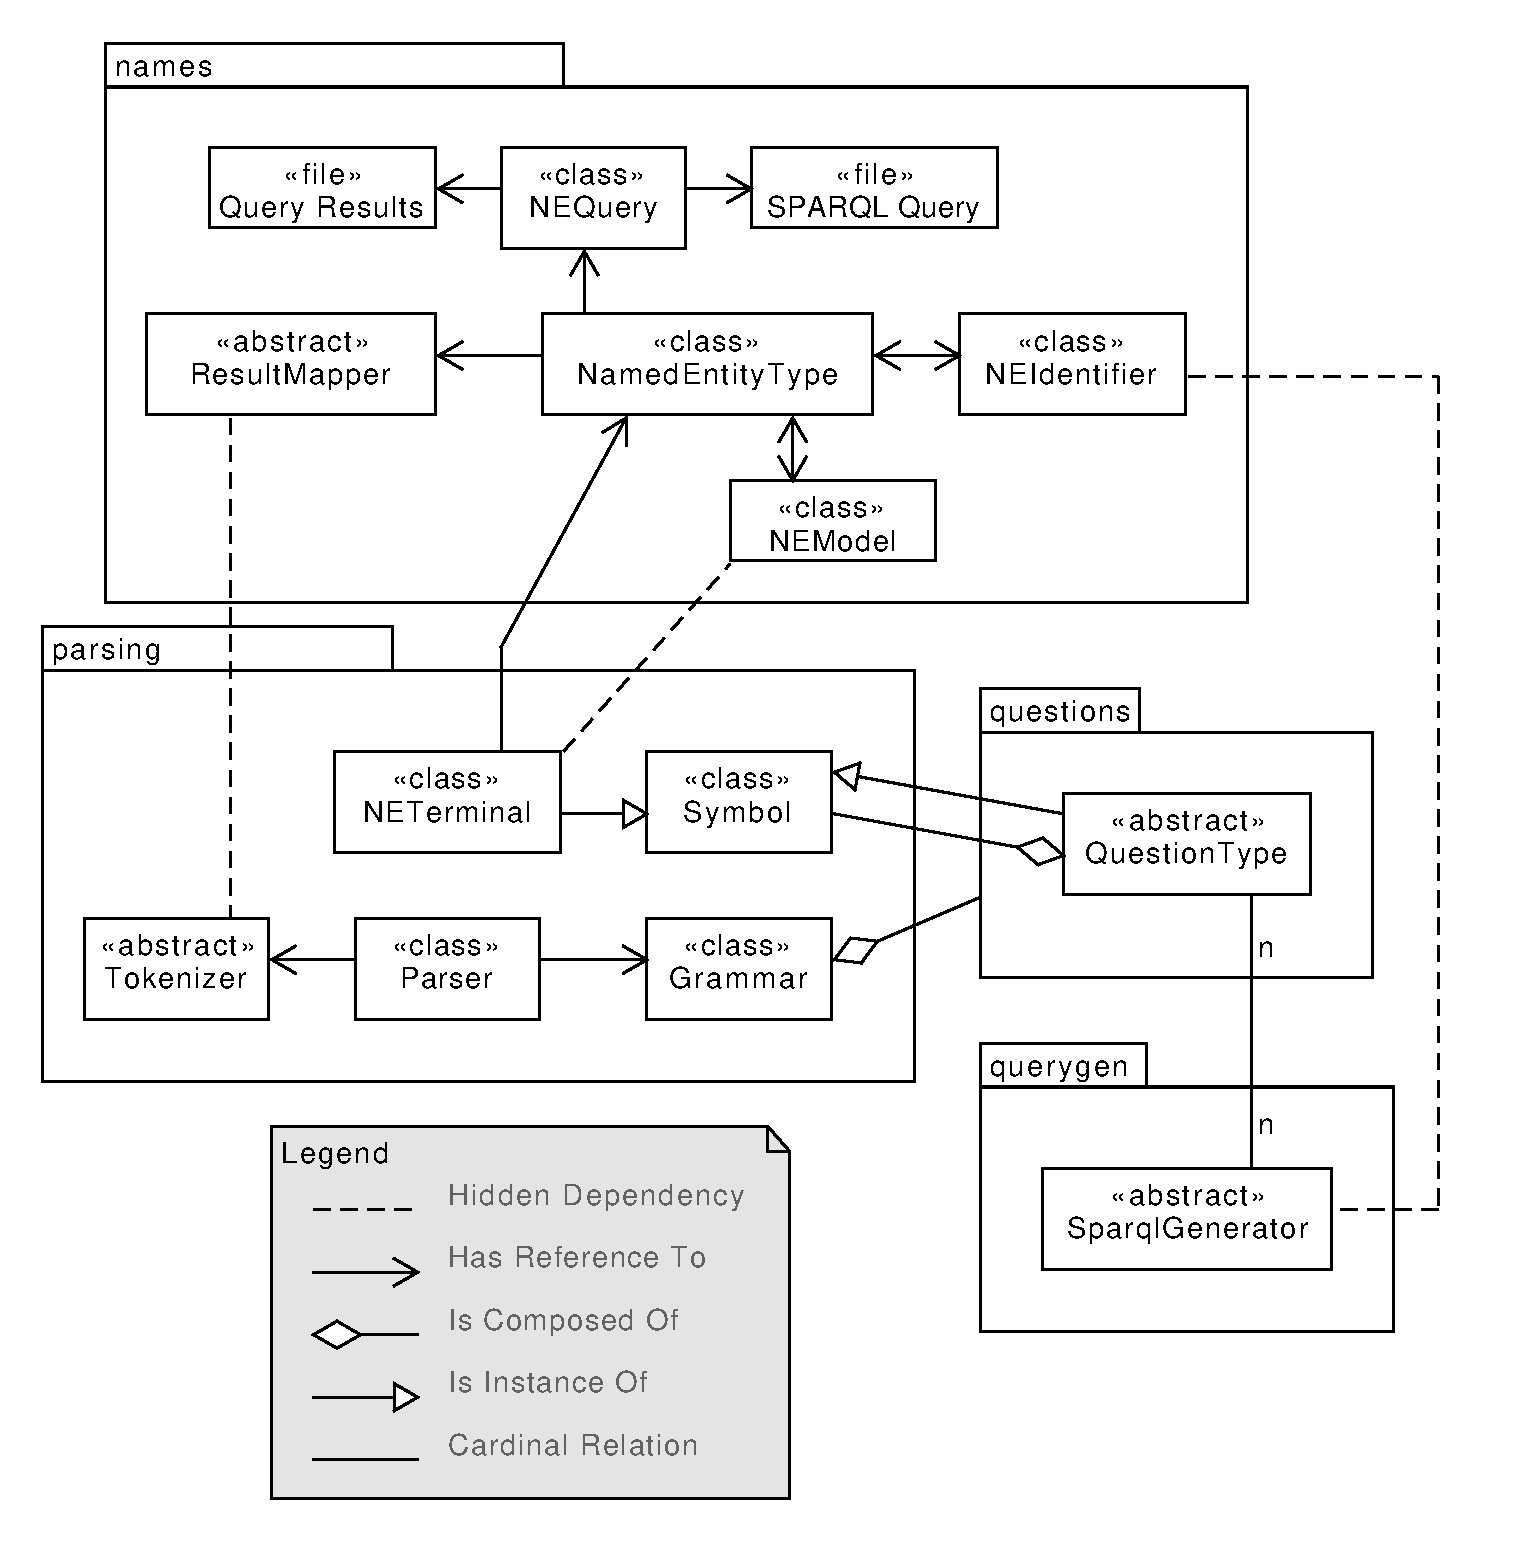
\includegraphics[width=0.9\textwidth,natwidth=1,natheight=1]{architecture.pdf}
    \caption{Architecture}
    \label{fig:arch}
\end{figure}


One of the goals of this project was to develop a
highly extensible architecture. There wasn't enough time to cover the
breadth of questions one would hope for in a mature product - such being
the nature of research. But I felt it was important to create a practical
working system that could handle a wide range of questions if more
time was dedicated towards that end.

To make the system extensible, it was important to decouple the various
components as much as possible. Still - language processing is a naturally
interdependent process with many overlapping concerns. For instance,
parsing seems to be an independent problem from named entity recognition (NER),
but to achieve better parsing results it was necessary to integrate NER into the
parser so that semantic context could inform the NER. 

\begin{figure}[h!]
    \centering
    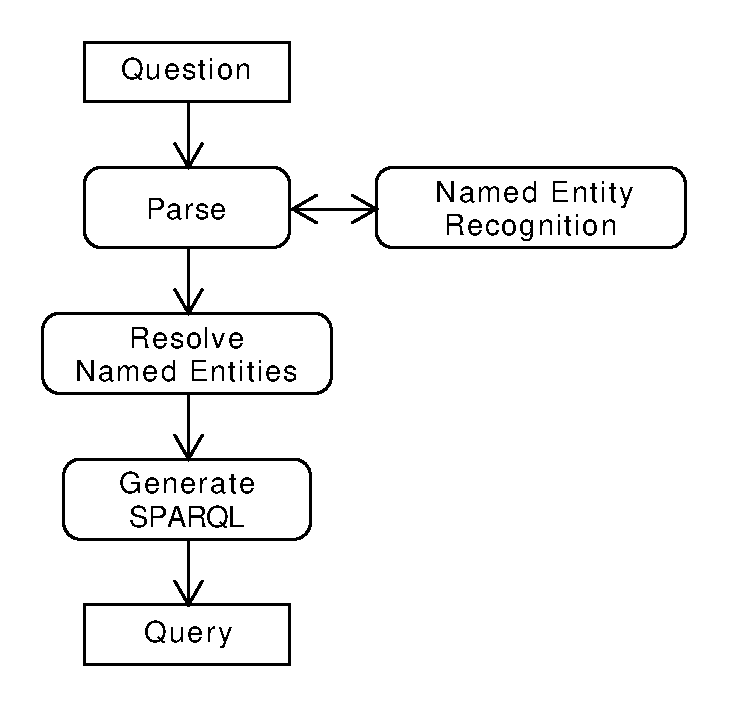
\includegraphics[width=0.5\textwidth,natwidth=1,natheight=1]{usage.pdf}
    \caption{Process}
    \label{fig:process}
\end{figure}

Another design concern was the accessability of the SPARQL endpoint.
It would be ideal if the endpoint was always accessable, would accept an unlimited
number of queries, and would always respond quickly. But in practice, none of
those ideals are true. As such, the results of certain queries
(necessary for developing NER models and URI resolution) are cached into local files.
The tradeoff is that data in the cache can stagnate. That problem is mitigated by 
simply flushing the cached results periodically.

\section{Named Entity Recognition}
Different types of named objects are recognized as part of the parsing process.
Since the names are matched durring parsing, the NER is greatly improved by context.
Still, this matching requires a bit of preprocessing.

Statistical character models are constructed from the output of queries for all 
objects of a certain type in the target RDF database. 
These models are used to recognize arbitrary tokens (or combinations of 
tokens) within the parser's grammar. 

These models allow for probablistic recognition of the input strings in 
$O(1)$ time (at least, in relation to the number of objects in the RDF
database). They recognize variations on the names (typos, variations, etc.)
within some user-defined bound. 

\section{Parsing, Resolution, and Compilation}
The parsing grammar is composed of rules to handle each type of question.
"Type of question" is ill defined, as it is largely a matter of design preference.
The broader the scope of a 'type', the harder it will be to develop a grammar
which recognizes that question. But the narrower the types, the more types
will need to be implemented to cover the same range of NL questions.

After parsing, specific instances of named entities need to be 'resolved' to
corresponding RDF entities. Natural language names (like "John Smith") are mapped
to RDF URIs (like "http://sbc.net/smith394")
algorithmically and with manual user aid. This boils down to searching a
database of names with a good fuzzy string matching algorithm and falling
back on the user to select the appropriate name when there is no single nearly-exact
match.

Compiling SPARQL queries from the resolved parse trees is the last step.
For each type of question, there will be a separate unit which 
generates SPARQL queries. There might be a more elegant way to handle this
problem, but this seems like an extensible (if tedious to implement) solution.
Generation is often just a matter of fitting RDF URIs into hard-coded templates.

%\bibliography{arch}{}
%\bibliographystyle{plain}
\end{document}
